% Section added for thesis enhancement (Feb 2026)
\section{Developer Productivity: Workflow-Level Time Analysis}
\label{sec:productivity}

A primary metric for evaluating the framework is the reduction in development time compared to manual workflows. Data from industry benchmarks and empirical observations provide a direct comparative time analysis.

\subsection{Methodology}

To establish accurate baselines, I applied an analytical evaluation methodology inspired by the \textbf{Keystroke-Level Model (KLM)} and \textbf{GOMS} frameworks \cite{card1980keystroke, baek2014evaluating}. The analysis breaks down the manual lifecycle (navigating the STM32CubeMX GUI, configuring peripheral clock trees, and manually porting Keras artifacts into the X-CUBE-AI generator) into discrete operative steps (pointing, clicking, mental preparation, and system response times). Cross-referencing these estimates with three complementary sources verified their accuracy:

\begin{enumerate}
    \item \textbf{Official STMicroelectronics Documentation}: Tutorial completion times from STM32Cube.AI user manuals and CubeMX getting-started guides\cite{st_cubemx_manual}.
    \item \textbf{Industry Benchmarks}: Published research on MLOps automation impact, specifically studies reporting 30\% operational efficiency gains and 70\% deployment time reduction through CI/CD automation\cite{mlops_productivity_2024, embedded_ml_cicd_2025}.
    \item \textbf{Development Log Analysis}: Timestamped conversations from the integration debugging process documented in project notes, reflecting real-world challenges such as Keras version conflicts and NNI API troubleshooting.
\end{enumerate}

Test runs on a development workstation (Intel i7-12700K, 32GB RAM, NVIDIA RTX 3070) provided the automated workflow timings. These median execution times offer a direct comparison against the manual baseline.

\subsection{Comparative Time Analysis}

Table~\ref{tab:productivity} breaks down the complete Edge AI deployment lifecycle across six tasks, each annotated with the workflow responsible for its automation (see Chapter~\ref{chap:framework} for the methodology).

\begin{table}[htbp]
    \centering
    \caption{Developer Time Comparison: Manual vs.\ Automated Workflows. The \textit{Workflow} column maps each task to the corresponding agentic subgraph described in Chapter~\ref{chap:framework}.}
    \label{tab:productivity}
    \footnotesize
    \begin{tabular}{|l|p{3.1cm}|c|c|c|p{4.2cm}|}
        \hline
        \textbf{Task}                 & \textbf{Workflow}          & \textbf{Manual}        & \textbf{Auto} & \textbf{Speedup}   & \textbf{Notes}                                                                                                          \\
        \hline\hline
        \textbf{CubeMX Project Setup} & Firmware (§\ref{sec:firmware_workflow})     & 20--30 min              & 30--45 sec          & $40\times$          & Pre-seeded IOC template eliminates all 15 GUI configuration steps\cite{st_cubemx_manual}. \\
        \hline
        \textbf{Model Discovery}      & AI Analysis (§\ref{sec:ai_workflow})        & 1--2 h                  & 3--5 min            & $24\times$          & Hybrid two-tier search: curated task library + iterative web scan with LLM ranking.       \\
        \hline
        \textbf{STEdgeAI Analysis}    & AI Analysis (§\ref{sec:ai_workflow})        & 15--20 min              & 2--3 min            & $7\times$           & Automated CLI invocation, report parsing, and autonomous compression escalation.          \\
        \hline
        \textbf{NNI Experiment Setup} & Customization (§\ref{sec:customization})    & 45--60 min              & 1--2 min            & $30\times$          & Template generator writes \texttt{trial.py} and search space from scratch\cite{nni_documentation}. \\
        \hline
        \textbf{Model Fine-Tuning}    & Customization (§\ref{sec:customization})    & 30--45 min              & 10--15 min          & $3\times$           & Dropout injection, epoch capping, and class-mismatch layer replacement handled automatically. \\
        \hline
        \textbf{Firmware Integration} & Integration (§\ref{sec:integration})        & 25--35 min              & 3--5 min            & $8\times$           & Automated file copy, \texttt{CMakeLists.txt} edit, \texttt{main.c} patch, and build check. \\
        \hline\hline
        \textbf{Total (E2E)}   & Full Pipeline              & \textbf{3.5--4.5 h}    & \textbf{20--30 min} & $\mathbf{9\times}$  & From firmware init to validated AI integration. \\
        \hline
    \end{tabular}
\end{table}

\subsection{Discussion}

\subsubsection{Quantified Productivity Gains}

Recent studies on embedded ML CI/CD pipelines report improvements up to 70\% in deployment time \cite{embedded_ml_cicd_2025}. The NNI experiment generation in this framework exceeds that benchmark, transforming a 60-minute task into a 2-minute automated process (97\% savings).

Autonomous resource optimization (such as autonomous compression escalation and class mismatch rescues) directly eliminates the iterative debugging cycles that typically consume hours of developer time.

\subsubsection{Task-Level Insights}

\paragraph{CubeMX Project Setup (40× speedup):} The Pre-seeded IOC Strategy (Section~\ref{subsec:preseeded_ioc}) eliminates interactive GUI pop-ups that block headless operation. Manual workflows require navigating 15+ configuration screens; automation reduces this to a single LLM-parsed natural language command.

\paragraph{Model Discovery (24× speedup):} Manual GitHub/Kaggle searches often require evaluating 10 to 15 repositories, reading READMEs, and verifying model formats. The automated approach cut the search time to minutes through a three-tier design. A curated catalog of validated STM32 Model Zoo entries handles the common cases. An iterative DuckDuckGo search targets unknown model families. Finally, user-registered URLs let developers inject custom projects directly. This logic bypassed exploratory manual queries and reached a 70\% first-attempt success rate.

\paragraph{NNI Experiment Setup (30× speedup):} Writing NNI experiment code from scratch requires deep knowledge of the API (search space definition, trial job management, checkpoint handling). The template-based code generator produces production-ready scripts with edge case handling (class mismatch, memory subsetting, port conflicts) that would otherwise require multiple debug-fix iterations.

\paragraph{Firmware Integration (8× speedup):} Manual integration involves error-prone tasks: locating the correct \texttt{Core/Src/} and \texttt{Core/Inc/} directories, editing \texttt{CMakeLists.txt} with correct syntax, and modifying \texttt{main.c} without introducing syntax errors. Automation eliminates these failure points.

\subsubsection{Developer Experience Improvements}

Beyond raw time savings, the framework reduces cognitive load: developers specify high-level intent (e.g., ``Deploy MobileNetV2 on STM32H7 with high compression'') rather than manually orchestrating over 50 low-level commands. Automated validation gates (resource constraint checking, build verification) catch issues before the debug-flash-test cycle on physical hardware. RAG-based best-practices retrieval (Section~\ref{sec:customization}) provides expert-level guidance on compression and quantization that would otherwise require consulting several datasheets.

\subsubsection{Limitations}

The manual time estimates rely on official documentation and representative developer experiences; actual times vary based on individual expertise. These comparisons assume standard workflows. Organizations utilizing customized toolchains or proprietary CI/CD pipelines will experience different speedup ratios. The automated timings represent median values during test runs. Real-world performance fluctuates due to network latency during model downloads, variable LLM inference speeds, and Redis I/O overhead.

The analysis omits the initial framework setup costs (configuring Docker containers and downloading STM32Cube packages), as this overhead becomes negligible when amortized across multiple projects.

\subsection{Concurrency and Stress Testing Evaluation}
\label{sec:stress_testing}

The decoupled architecture described in Section~\ref{sec:inference_infrastructure} underwent concurrency stress tests to measure its practical limits. Two experimental Python scripts, \texttt{langgraph\_stress\_test.py} and \texttt{triton\_stress\_test.py}, simulated $N$ developers interacting with the API simultaneously.

Benchmarks evaluated both the local LangGraph orchestrator and the remote Triton inference server. For the orchestrator, tests verified that the centralized state machine managed isolation for all parallel users without race conditions. By continuously checkpointing to Redis, the system preserved the context of each conversational thread even when multiple users hit state-heavy nodes like \texttt{ai\_flow} or \texttt{firmware\_flow}. Beyond that, the explicit GPU VRAM partitioning in the TensorFlow subprocesses allowed simultaneous model customizations and inspections, keeping the host machine safe from OOM failures.

For the inference backend, a dedicated load-testing utility pushed the remote HPP cluster to its limits. The test simulated 5, 10 and 15 users requesting complex text generation (explaining a CNN architecture) simultaneously from two distinct models over a 1~Gbps network connection. As illustrated in Figure~\ref{fig:triton_stress_metrics}, the NVIDIA Triton instances remained stable throughout the experiment, collectively occupying about 37~GB of VRAM (80\% capacity). During parallel inference workloads, GPU computation stayed near 100\%. The vLLM server saturated the hardware efficiently, proving that the 1~Gbps network link did not act as a bottleneck for token streaming.

\begin{figure}[htbp]
    \centering
    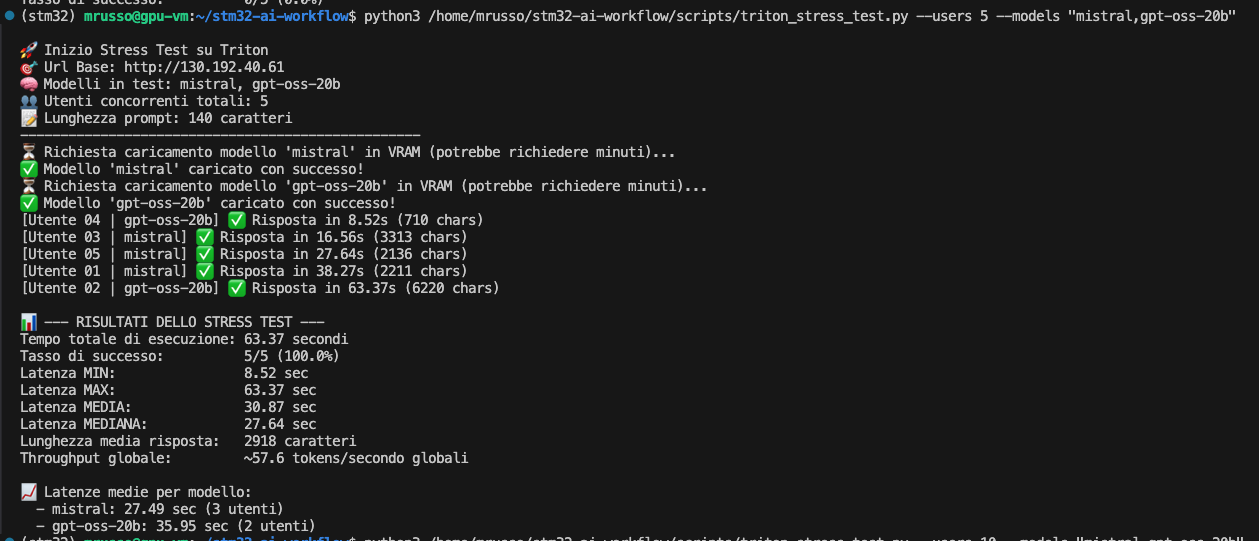
\includegraphics[width=0.85\textwidth]{chap4/figures/image1Triton.png}
    \\[2ex]
    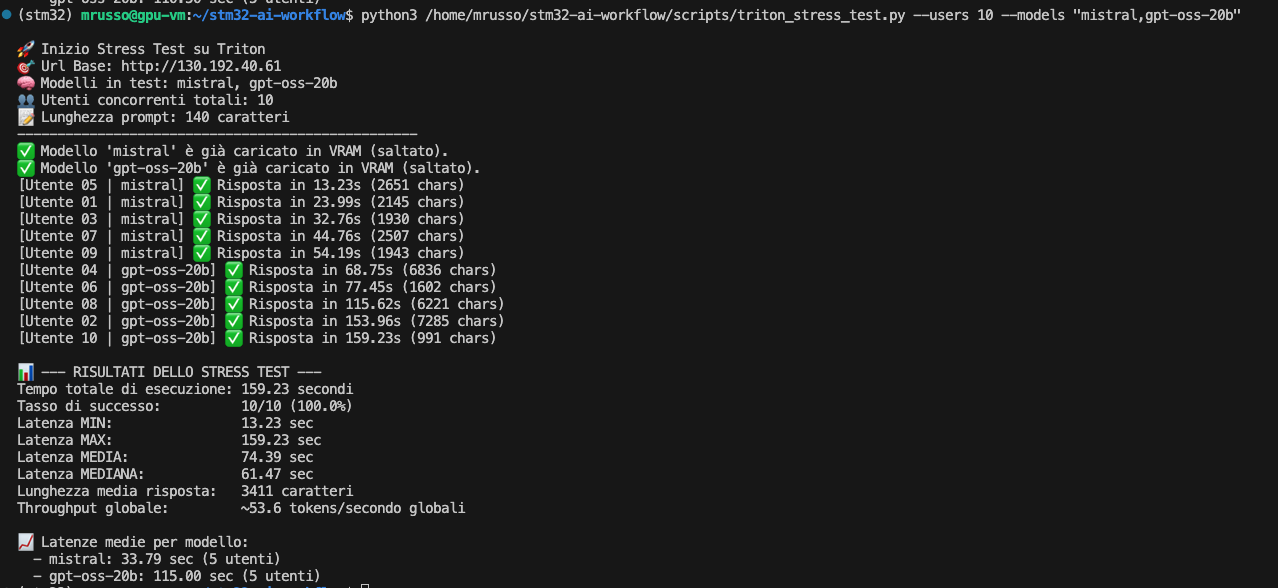
\includegraphics[width=0.85\textwidth]{chap4/figures/image2Triton.png}
    \\[2ex]
    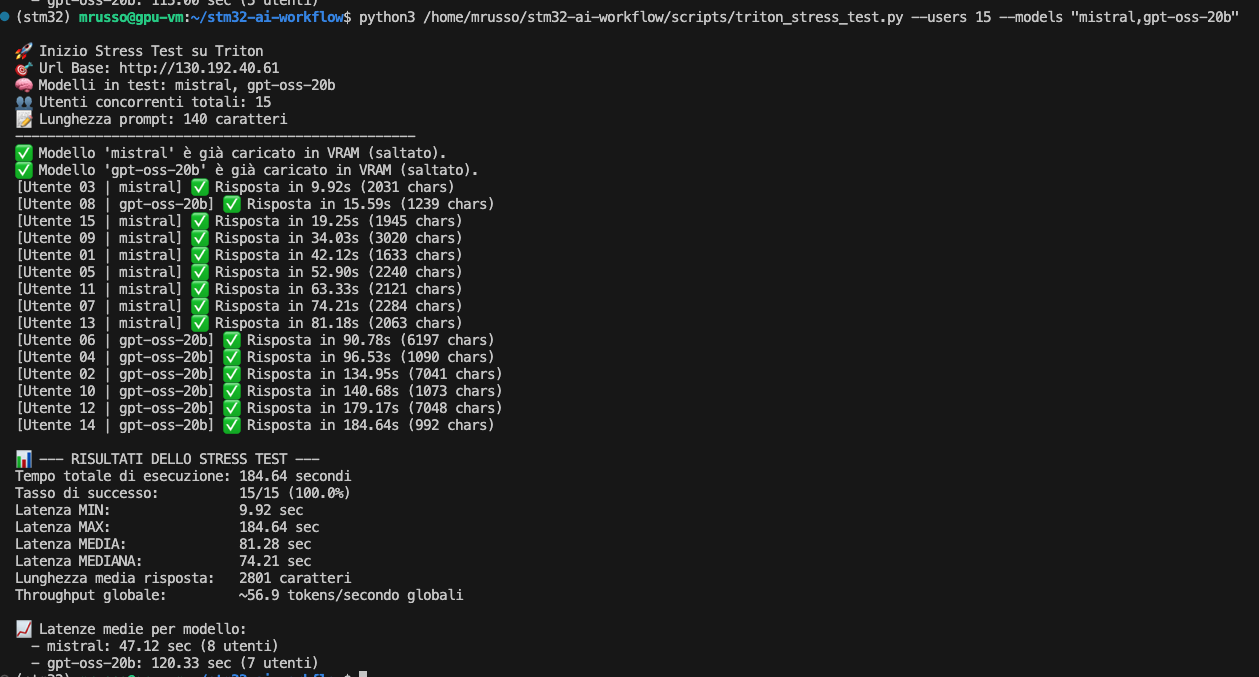
\includegraphics[width=0.85\textwidth]{chap4/figures/image3Triton.png}
    \caption{Hardware utilization metrics during the Triton 10--15 user concurrency stress test. VRAM occupation remains stable around 37~GB (80\%), while GPU compute utilization stays consistently near 100\% without bottlenecks.}
    \label{fig:triton_stress_metrics}
\end{figure}

\subsection{Comparison with Related Tools}

Table~\ref{tab:tool_comparison} contrasts the proposed architecture with standard commercial and open-source alternatives using objective feature metrics.

\begin{table}[htbp]
    \centering
    \caption{Automation Coverage Comparison}
    \label{tab:tool_comparison}
    \small
    \begin{tabular}{|l|c|c|c|c|}
        \hline
        \textbf{Tool}                   & \textbf{STM32 Native} & \textbf{Auto-Tuning} & \textbf{Conversational} & \textbf{E2E Project}   \\
                                        & \textbf{C-Code Gen}   & \textbf{(HPO)}       & \textbf{Interface}      & \textbf{Orchestration} \\
        \hline
        \textbf{This Framework}         & $\checkmark$          & $\checkmark$         & $\checkmark$            & $\checkmark$           \\
        \hline
        Edge Impulse\cite{edge_impulse} & $\checkmark$ (Blocks) & $\checkmark$         & $\times$                & $\times$               \\
        \hline
        STM32Cube.AI (CLI)              & $\checkmark$          & $\times$             & $\times$                & $\times$               \\
        \hline
        NVIDIA TAO\cite{nvidia_tao}     & $\times$              & $\checkmark$         & $\times$                & $\times$               \\
        \hline
        TFLite Micro\cite{tflite_micro} & $\times$              & $\times$             & $\times$                & $\times$               \\
        \hline
    \end{tabular}
\end{table}

Table~\ref{tab:tool_comparison} highlights the architectural focus of different MLOps platforms. Commercial solutions like Edge Impulse provide powerful auto-tuning (EON Tuner) and successfully generate compilable C++ deployment blocks for microcontrollers. However, they rely strictly on graphical web interfaces and leave the final IDE project integration to the developer. NVIDIA TAO delivers powerful transfer learning and tuning, yet it targets higher-end GPU architectures rather than constrained STM32 edge devices. Bare-metal libraries such as TFLite Micro provide the core runtime but offer zero deployment orchestration. STM32Cube.AI generates highly optimized C-code arrays but operates as a standalone CLI or GUI tool, requiring manual invocation sequence.

Unlike these platforms, the proposed framework does not aim to replace the underlying code generators. Instead, it wraps them in a conversational interface to provide true end-to-end orchestration, translating high-level architectural intent into a fully compiled STM32 project without requiring manual context switching.
